\section{Theorie}

\subsection{Stubfilter}

LC-Filter können in einem weiten Frequenzbereich eingesetzt werden. Jedoch wird bei konzentrierten Elementen zu höheren Frequenzen hin der Einfluss der parasitären Eigenschaften immer deutlicher, so dass hohe Anaforderungen an die Bauteilgüte gestellt werden müssen. Im GHZ-Bereich wird es daher zunehmend attraktiv, statt konzentrierten Kapazitäten und Induktivitäten verteilte Strukturen in Form von Leitungen zu verwenden.Es handelt sich dabei um sogenannte Leitungsfilter.
%Quelle direktes Zitat: 
%https://books.google.ch/books?id=MTVQAgAAQBAJ&pg=PA203&lpg=PA203&dq=leitungsfilter+hochfrequenztechnik&source=bl&ots=Ljf0GRJkZt&sig=n-0G9H5VZ9iuPc2qepAATnjA47M&hl=de&sa=X&ved=0ahUKEwj38u-T79DUAhUSL1AKHUsyDNMQ6AEINTAB#v=onepage&q=leitungsfilter%20hochfrequenztechnik&f=false%

Es gibt verschiedene Arten um Leitungsfilter zu realisieren. Eine Möglichkeit der Realisierung ist das Stubfilter. Dieses Filter verwendet gleichlange kurzgeschlossenen Leitungen (TLSC) und leerlaufende Leitungen(TLOC), die nur an einem Ende verbunden werden. Das andere Ende wird entweder kurzgeschlossen oder eben offen gelassen. Bei diesen Leitungen handelt es sich um sogennante Stubs(Stichleitungen), die sich bei hohen Frequenzen wie reaktive Elemente (L,C) verhalten und somit die Realisierung eines Mikrowellenfilter ermöglichen.
Damit ein Ingenieur in der Lage ist ein Stubfilter korrekt zu dimensionieren, muss er zuerst das allgemeine Vorgehen bei einer Filterdimensionierung verstehen. Dieses Vorgehen ist unabhängig vom zu realisierenden Filter und wird im folgenden Kapitel näher beschrieben.
 
%Der grosse Vorteil von Stubfiltern ist, das eine geschlossene Theorie zur Filtersynthese existiert. Um diese Theorie verstehen zu können wird vorerst die 

\newpage


\subsection{Ablauf Filterdimensionierung}

Der Entwurfsprozess jedes Filters (Abb.\ref{fig:Ablauf_Filterdimensionierung}) beginnt mit der  Filterspezifikation, welche mathematisch mit einer Funktion im Prototypbereich T(s) beschrieben wird. Aus dieser Funktion kann mit Hilfe einer Filtersynthese eine realisierbare Filterstruktur gefunden werden. Dabei ist zu beachten, dass  physikalische Randbedingungen einbezogen werden müssen, die nicht beliebig steile und beliebig verlustfreie Filtercharakteristiken erlauben.

Die Filtersynthesen unterschiedlicher Filter-Realisierungen haben gemeinsam, dass sie alle auf der klassischen LC-Filtersynthese basieren. Nach der LC-Filtersynthese liegt ein LC-Prototypfilter vor, welches mithilfe von unterschiedlichen Transformationen in einen andere Filter-Typ überführt werden kann. Bekannte Transformationen sind z.B die billineare, impulsinvariante oder die Kuroda-Transformation.

\begin{figure}[h!]
\centering
 	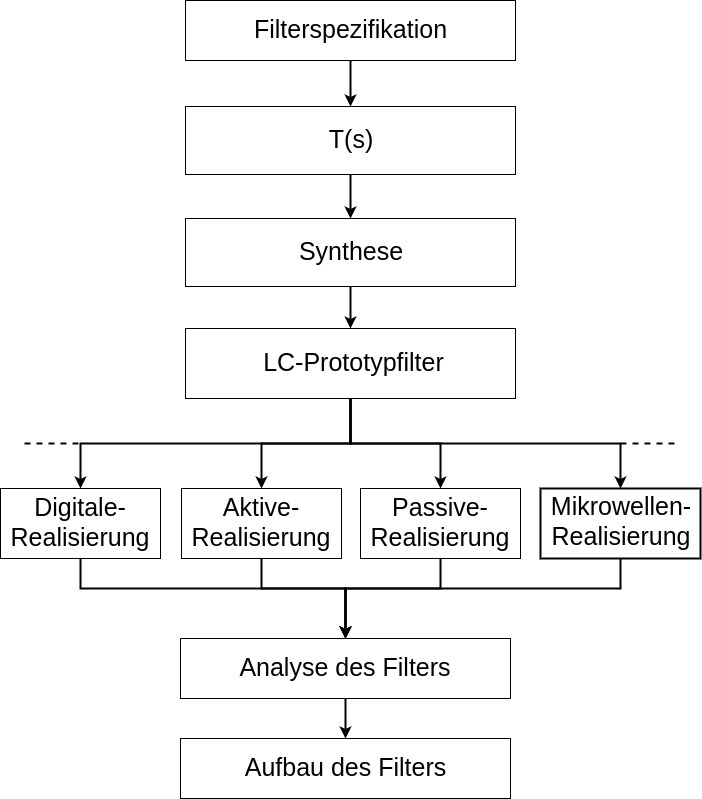
\includegraphics[width=0.5\textwidth]{Ablauf_Filterdimensionierung_Allgemein.png}
 	\caption{Ablauf Filterdimensionierung}
 	\label{fig:Ablauf_Filterdimensionierung}
\end{figure}



%Liegen keine speziellen Anforderungen an das Filter vor, so können Standardfilter(Butterworth, Chebyshev, Bessel und Cauer)verwendet werden. Die Reaktanzwerte, welche für die Beschreibung der Übertragungsfunktion des LC-Prototypfilters notwendig sind, sind aus Tabellen zu entnehmen. Werden Spezielle Anforderungen an das Filter gestellt, so eignen sich die Standardfilter nicht und es muss eine LC-Filtersynthese durchgeführt werden.


\subsection{Ablauf Stubfilterdimensionierung}



%In diesem Kapitel wird erläutert, wie bei der Dimensionierung eines Stubfilters  vorgegangen wird. Der typische Ablauf zur Dimensionierung eines Stubfiltern ist in Abb. \ref{fig:Ablauf_Filterdimensionierung dargestellt. Dieser Ablauf unterscheidet sich nicht gross vom Ablauf bei der Dimensionierung eines digitalen oder  Ablaufwird auch für die Realisierung von aktiven, passiven und digitalen Filters verwendet. Der einzige Unterschied ist, dass sich die Schritte in Filter-Realisierung(blau umrandet) unterscheiden.

Ausgangslage für jede Filterdimensionierung ist die Filterspezifikation, welche im Frequenz- oder Zeitbereich vorliegt. Diese Filterspezifikation wird anschliessen mathematisch mit einer Funktion in der s-Ebene (Prototypbereich) beschrieben. Mit einem Synthesetool kann aus der Funktion in der s-Ebene ein Prototypfilter mit konzentrierten Elementen(R,L,C) gefunden werden. Dabei gibt das Synthesetool die Topologie, sowie die Bauteilwerte aus. Liegt kein Synthesetool vor, so müssen Standardfilter (Butterworth, Chebyshev, Bessel und Cauer) verwendet werden, deren Topologie und Bauteilwerte normiert aus einer Tabelle zu entnehmen sind. Bei sehr speziellen Anforderungen an das Filter reichen die Standardfilter aber meist nicht aus um die Filterspezifikationen einzuhalten.

Nach der Synthese liegt nun ein Prototypfilter mit konzentrierten Elementen vor, gesucht ist aber ein Stubfilter, welches aus verteilten Elementen (Leitungen) besteht. Hier kommt die Frequenztransformation von Richards zum Zuge. Richards konnte zeigen, dass sich gleichlange, verlustlose Leitungen (TLSC,TLOC) gleich wie konzentrierte Elemente verhalten, wenn die folgende Transformation für die laplace variable verwendet wird.

s= dhsijdkh

Mit der Frequenztransformation von Richards kann dieses Filter vom Prototypbereich(s-Eben) in den Originalbereich (f-Ebene) transformiert werden. Dadurch werden die konzentrierten Elemente(L,C) in verteilte Elemente (Leitungen) umgewandelt. Dies 
TLSC = ideale, verlustlose Transmission Line im kurzschluss
TLOC = ideale, verlustlse Tranmissin Line im Leerlauf



\newpage

\begin{figure}[h!]
\centering
 	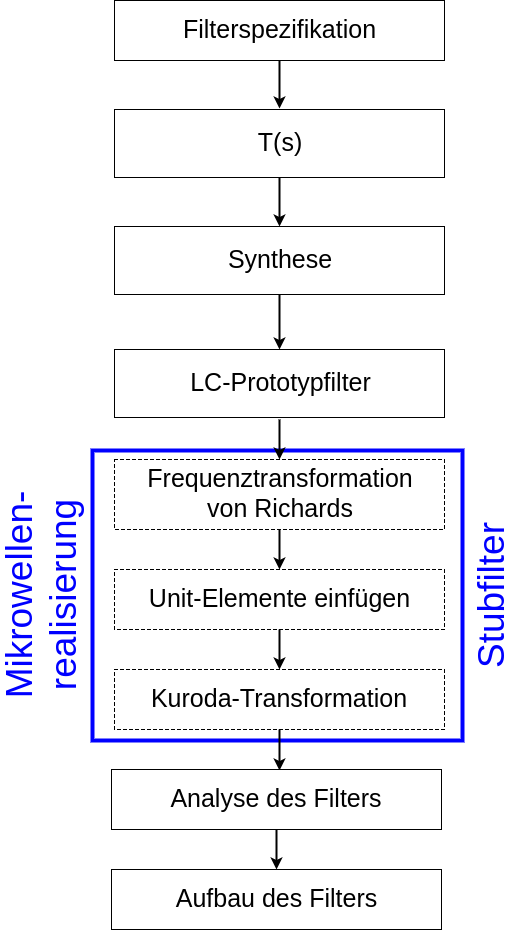
\includegraphics[width=0.5\textwidth]{Ablauf_Filterdimensionierung.png}
 	\caption{Ablauf der Stubfilter-Dimensionierung}
 	\label{fig:Ablauf_Filterdimensionierung}
\end{figure}















%Die "Übersetzung" von klassischen LC-Filtern in Leitungsfilter kann meist problemlos und rein routinemässig vorgenommen werden. Leider resultieren dabei häufig Filterstrukturen, die beispielsweise mit Mikrostreifenleitungen nicht ausführbar sind, da diese einen nur sehr eingeschränkten Bereich der Wellenimpedanz zulassen. So lässt z. B. ein AJumina-Substrat (Er = 10) nur einen Bereich der Wellenimpedanz von Zw = 20 ... 100 n mit vernünftigen Leiterbreiten zu. Die Kunst des Filterentwurfs liegt also darin, den richtigen, mit der gewählten Technik realisierbaren Filtertyp zu finden.


Diese Einführung zum Entwurf von Leitungsfiltem der Höchstfrequenztechnik umfasst folgen-
de Teile:
1. Einführung zu Butterworth- und Tschebyscheff-Filtern. Filterentwurf mit Standardtief-
pässen.
2. Die Richards-Transformation, welche erlaubt, ein LC-Filter in einen Typ von Leitungsfil-
ter überzuführen (Filter mit kommensurablen Leitungen).
3. Die Kuroda-Transformation, welche einen Teil der Richards-transformierten Filter in rea-lisierbare Mikrostreifenfilter umzuwandeln vermag.
4. Schmalbandige Bandpässe mit Leitungselementen als Impedanzinverter.


%Bärchtold






